\documentclass[11pt]{article}

% --- packages -------------------------------------------------------------
\usepackage[a4paper,margin=1in]{geometry}
\usepackage[utf8]{inputenc}
\usepackage[T1]{fontenc}
% Emit a ToUnicode map so PDF text extraction / copy-paste resolves ligatures
% (fi, fl, ...) correctly with the default fonts (arXiv-recommended; no lmodern
% needed). Must precede the document body.
\input{glyphtounicode}
\pdfgentounicode=1
\usepackage{amsmath}
\usepackage{booktabs}
\usepackage{graphicx}
\usepackage[table]{xcolor}
\usepackage{caption}
\usepackage{enumitem}
\usepackage[expansion=false]{microtype}  % char protrusion (expansion needs scalable fonts)
\usepackage[hidelinks]{hyperref}
\usepackage{xurl}  % allow long URLs to break across lines (no margin overflow)

\definecolor{mocblue}{HTML}{1A73E8}
\graphicspath{{figures/}}

% --- metadata -------------------------------------------------------------
\title{\textbf{Matrix Context: Mixture-of-Contexts RAG for Robust and
Inspectable Agent Memory}\\[0.3em]
\large Routing typed context experts improves robustness under paraphrased and
adversarial queries}

\author{Ruslan Magana Vsevolodovna\\
\small Independent Researcher, Genova, Italy \\
\small \texttt{contact@ruslanmv.com} \,$\cdot$\, \href{https://ruslanmv.com}{ruslanmv.com}}

\date{June 2026}

\begin{document}
\maketitle

\begin{abstract}
We introduce \emph{Mixture-of-Contexts RAG} (MoC-RAG), a routed retrieval
architecture for agent memory that selects a small set of \emph{typed context
experts} \emph{before} retrieving, then assembles a token-budgeted,
inspectable context pack. To test the architecture beyond a keyword-aligned
fixture, we build a public benchmark of typed agent memory (1{,}000 context
items, 600 queries, eight experts, six domains) in which every gold fact is
surrounded by five kinds of \emph{hard negative} and queried in five styles
ranging from direct to adversarial, with the same test topics phrased into
parallel \texttt{keyword}, \texttt{paraphrased}, and \texttt{adversarial}
splits. On this benchmark MoC-RAG improves robustness over flat RAG baselines:
under adversarial lexical shift a strong lexical baseline (BM25) drops from
100\% to 64\% Recall@8 ($-36$ points), whereas MoC-RAG holds within $\sim$17
points and overtakes BM25 on the adversarial split by $\sim$15 points, while
carrying roughly half the hard distractors of dense, hybrid, metadata-filtered,
and reranked RAG at 95--100\% expert-routing accuracy. We are careful not to
overclaim: BM25 remains strong on keyword-aligned queries, and MoC-RAG's
advantage is robustness and context efficiency under typed, distractor-heavy,
paraphrased and adversarial conditions---the regime real agent memory inhabits.
All figures and tables in this paper are regenerated from committed result
artifacts by the accompanying scripts.
\end{abstract}

\section{Introduction}

Retrieval-augmented generation~\cite{lewis2020rag} has largely settled into one
pattern: embed everything into a single flat index and retrieve the nearest
chunks for every query. For agent memory---where the store mixes user
preferences, project decisions, code, policies, episodes, and documents---this
is both wasteful and opaque. It spends a fixed prompt budget without regard to
the \emph{type} of what it retrieves, and it offers no account of \emph{why} a
given item was chosen.

Matrix Context proposes a different shape, which we call
\emph{Mixture-of-Contexts RAG} (MoC-RAG). Rather than retrieving from one
undifferentiated store, it routes each query to the smallest useful subset of
typed \emph{context experts}, retrieves with a hybrid lexical and dense fusion
inside them, and assembles a token-budgeted pack scored by relevance,
importance, recency, and a redundancy penalty---with every selection explainable
through an \texttt{inspect} interface.

The central question is empirical and easy to get wrong. On queries whose words
overlap the gold answer, a strong lexical baseline such as BM25~\cite{robertson2009bm25}
is hard to beat, and any apparent routing win could simply reflect easy
retrieval. We therefore stress-test the architecture where lexical matching
becomes unreliable---under paraphrase and under \emph{adversarial} queries that
embed misleading terms. Figure~\ref{fig:recall_by_type} previews the headline:
BM25 is excellent on keyword-aligned queries and brittle under adversarial
shift, while MoC-RAG degrades far more gracefully.

\paragraph{Contributions.}
\begin{enumerate}[leftmargin=1.4em,itemsep=2pt]
  \item \textbf{MoC-RAG}, a routed retrieval architecture with a hybrid expert
  router (centroid + keyword + type + scope + activity priors) and an
  inspectable, budgeted pack assembler (\S\ref{sec:method}).
  \item A \textbf{public typed agent-memory benchmark} with five hard-negative
  kinds and five query styles, including parallel keyword / paraphrased /
  adversarial test splits that isolate robustness from topic leakage
  (\S\ref{sec:benchmark}).
  \item An \textbf{evidence-based robustness result}: MoC-RAG preserves higher
  recall under adversarial lexical shift and roughly halves hard distractors
  versus the dense baseline family, at 95--100\% routing accuracy
  (\S\ref{sec:results}), together with a fully reproducible figure/table
  pipeline.
\end{enumerate}

\begin{figure}[t]
  \centering
  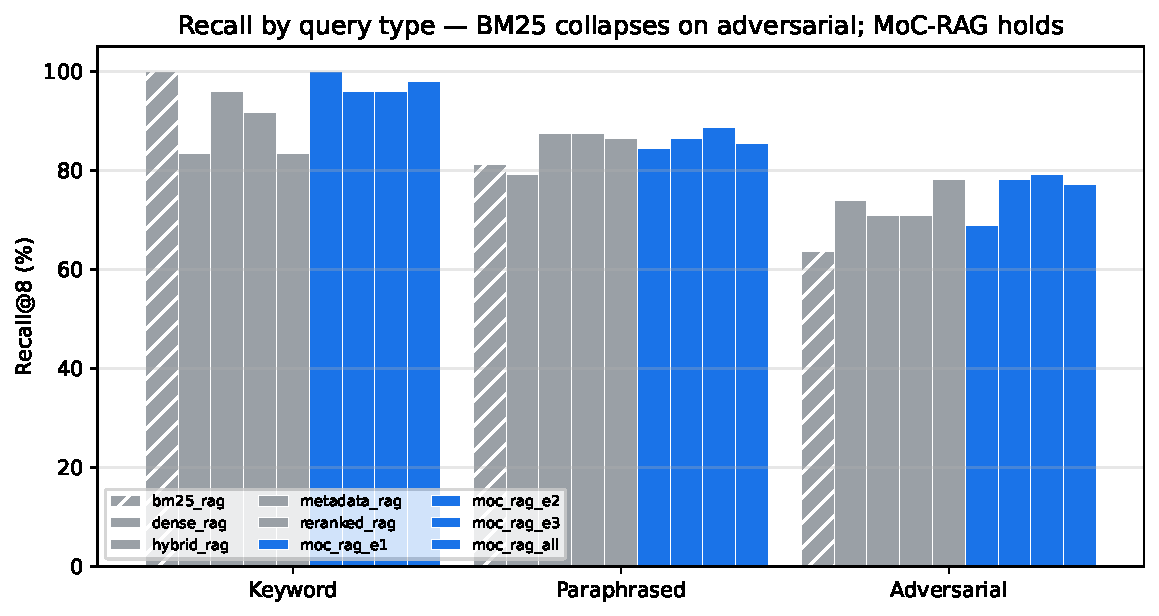
\includegraphics[width=\linewidth]{recall_by_query_type.pdf}
  \caption{Recall@8 by query type (sentence-transformers embedder). BM25 leads
  on keyword-aligned queries but collapses under adversarial phrasing; MoC-RAG
  variants hold and overtake it on the adversarial split.}
  \label{fig:recall_by_type}
\end{figure}

\section{Background and Related Work}

\paragraph{Sparse routing.} The organizing principle behind MoC-RAG is sparse
routing: expose many specialists but activate only the few a given input
requires. This is the mechanism by which mixture-of-experts models scale
capacity without proportional compute~\cite{shazeer2017moe}. Matrix Context
applies the same principle not to model weights but to \emph{context}, treating
the memory store as a set of typed experts selected per query.

\paragraph{Retrieval and fusion.} Classic dense RAG~\cite{lewis2020rag} retrieves
nearest neighbours from one index; lexical retrieval via BM25~\cite{robertson2009bm25}
remains a strong, hard-to-beat baseline when query and target share vocabulary.
Hybrid systems combine the two; we fuse the lexical and dense rankings with
Reciprocal Rank Fusion~\cite{cormack2009rrf}, which needs no score calibration
between channels. Dense embeddings are computed with
sentence-transformers~\cite{reimers2019sbert}. Redundancy in the assembled pack
is controlled with a maximal-marginal-relevance penalty~\cite{carbonell1998mmr}.

\paragraph{Is this just metadata filtering?} A natural objection is that routing
to typed experts is equivalent to filtering a flat index by metadata. We treat
this head-on by including a metadata-filtered hybrid RAG baseline that filters
candidates by the query scope before retrieving (\S\ref{sec:benchmark}). MoC-RAG
differs in two ways: it routes by \emph{learned and prior-weighted typed
relevance} rather than a hard metadata predicate, and it widens its expert
selection under uncertainty rather than returning an empty or wrong-typed set.
The benchmark measures whether this matters.

\paragraph{Agent memory.} The contemporary agent-memory landscape---personalization,
temporal knowledge graphs, operating-system-style memory management for
long-running agents, and graph reasoning over private corpora---reflects the
state of the field in early 2026. Matrix Context does not claim benchmark
supremacy over these systems; its position is a narrower combination they do not
bundle: a local-first default, typed and inspectable routing, and native fit
within a single agent ecosystem.

\section{Method: Matrix Context / MoC-RAG}
\label{sec:method}

MoC-RAG is a four-stage pipeline---route, retrieve, rerank, pack---over a store
of typed context items, with every stage exposed for inspection
(Figure~\ref{fig:architecture}).

\begin{figure}[t]
  \centering
  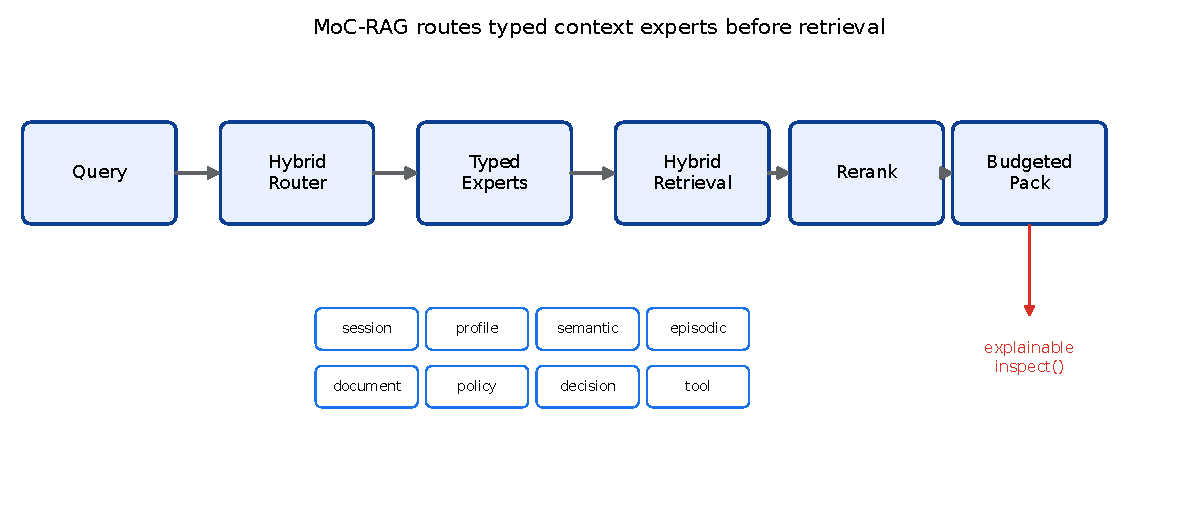
\includegraphics[width=\linewidth]{architecture.pdf}
  \caption{MoC-RAG routes a query to typed context experts before retrieving,
  then reranks and packs under a token budget; every choice is explainable.}
  \label{fig:architecture}
\end{figure}

\paragraph{Typed context items.} The unit of memory carries content, an
\emph{expert} partition, a \emph{type}, a hierarchical scope, an author-set
importance, a confidence, an optional time-to-live, and an embedding. Typing the
item is what enables routing by meaning and, later, governance by policy.

\paragraph{Hybrid expert router.} Given a query $q$ the router scores each expert
$e$ as a weighted sum of a dense centroid similarity and four cheap priors:
\begin{equation}
\mathrm{score}(e) = 0.40\,\mathrm{cos}(q, c_e) + 0.25\,\mathrm{kw}(q,e)
 + 0.15\,\mathrm{type}(q,e) + 0.10\,\mathrm{scope}(q,e) + 0.10\,\mathrm{act}(e),
\end{equation}
where $c_e$ is the expert centroid (mean item embedding blended with a seed
description), $\mathrm{kw}$ is keyword-prior overlap, $\mathrm{type}$ a query-intent
type prior, $\mathrm{scope}$ a scope-membership prior, and $\mathrm{act}$ a recent-activity
prior. The top-$k$ experts are selected; on low confidence or an indecisive
margin the router \emph{widens} selection rather than guessing---graceful
degradation that is exactly the seam where a learned classifier later plugs in.

\paragraph{Hybrid retrieval.} Within the selected experts, candidates are ranked
by Reciprocal Rank Fusion~\cite{cormack2009rrf} of a BM25 channel and a dense
channel, so a weak channel cannot dominate.

\paragraph{Reranking.} An optional local reranker re-scores the fused candidates
by a normalized blend of dense, lexical, importance, confidence, and recency,
leaving a cross-encoder seam for stronger rerankers.

\paragraph{Budgeted pack assembly.} The pack is filled greedily under a token
budget by
\(
s(i) = w_R\,\mathrm{rel}(i) + w_I\,\mathrm{imp}(i) + w_T\,\mathrm{rec}(i)
 - w_D\,\mathrm{red}(i),
\)
where the redundancy term is a maximal-marginal-relevance penalty~\cite{carbonell1998mmr}
that deduplicates near-identical memories at read time. Every kept and dropped
item, its score breakdown, and the routing reason are returned by
\texttt{inspect}, so the resulting context is auditable rather than a black box.

\section{Benchmark Design}
\label{sec:benchmark}

A small feasibility fixture is enough to show the mechanism but too
keyword-aligned to settle the obvious objection. We therefore build a larger,
public benchmark of typed agent memory, designed so that lexical overlap can be
dialed down deliberately (Table~\ref{tab:dataset}).

\begin{table}[t]
  \centering
  \caption{MoC-RAG Benchmark statistics (deterministically generated).}
  \label{tab:dataset}
  \begin{tabular}{l r}
\toprule
Statistic & Value \\
\midrule
Context items & 1000 \\
Queries & 600 \\
Context experts & 8 \\
Context types & 10 \\
Domains & 6 \\
Query variants & 5 \\
Hard-negative kinds & 5 \\
Train / Val / Test queries & 360 / 120 / 120 \\
Adversarial test queries & 48 \\
\bottomrule
\end{tabular}

\end{table}

\paragraph{Typed items and domains.} The store spans six agentic-memory
domains---project architecture, user/persona, code context, policy rules,
tool/session history, and document QA---mapped onto eight typed experts and ten
context types. Items carry importance, confidence, scope, and timestamps.

\paragraph{Hard negatives.} Each gold fact is surrounded by five kinds of hard
negative, the cases where flat retrieval is tempted: \emph{same keyword, wrong
expert}; \emph{true fact, wrong scope}; \emph{outdated (superseded) decision};
\emph{contradictory memory}; and \emph{stale session note}.

\paragraph{Query variants.} Crucially, every gold fact is queried five ways while
the gold label is held constant: \texttt{direct} (keyword-aligned),
\texttt{paraphrased}, \texttt{underspecified}, \texttt{cross\_expert}, and
\texttt{adversarial}. The adversarial phrasing deliberately embeds a misleading
term---the same value asserted by the contradictory negative---so a flat
lexical or dense retriever is genuinely lured toward the wrong item.

\paragraph{Parallel robustness splits.} Splitting is performed at the
\emph{topic} level, so all variants of a topic stay in one bucket. The test
topics are then phrased three ways into parallel \texttt{test\_keyword},
\texttt{test\_paraphrased}, and \texttt{test\_adversarial} splits. Because the
three splits cover the same topics, a change in score is attributable to query
\emph{style} rather than to topic leakage---this is what licenses the robustness
comparison in \S\ref{sec:results}.

\paragraph{Baselines.} We compare BM25, dense, hybrid (BM25$+$dense RRF),
metadata-filtered hybrid, and reranked RAG against MoC-RAG with
$\mathrm{top\_experts}\in\{1,2,3,\mathrm{all}\}$. All methods share one budgeted
packer, so differences reflect retrieval and routing quality, not packer tricks.

\section{Experiments}
\label{sec:experiments}

\paragraph{Setup.} We evaluate with two embedders: an offline zero-dependency
hashing embedder (a continuous-integration guard that requires no model
download) and \path{sentence-transformers/all-MiniLM-L6-v2}~\cite{reimers2019sbert}
as the competent embedder. Unless stated otherwise, results use the real
embedder, a per-query token budget of 200, and $K=8$ for ranking metrics. Each
method indexes the same 1{,}000-item store and is evaluated on the held-out test
queries.

\paragraph{Metrics.} We report retrieval quality (Recall@$K$, Precision@$K$,
MRR, nDCG@$K$), context efficiency (packed \emph{hard distractors}, total tokens,
useful-context ratio, and Recall@$K$ per 1k tokens), expert routing accuracy for
routed methods, and latency. \emph{Hard distractors} count items from a query's
labeled hard-negative set that enter the assembled pack---the harmful context a
good router should keep out.

\paragraph{Reproducibility.} The benchmark is deterministic (seeded) and every
number, figure, and table in this paper is regenerated from committed result
artifacts:
{\small
\begin{verbatim}
python -m benchmarks.moc_rag_benchmark.run build
python -m benchmarks.moc_rag_benchmark.run run     --split test --embedder st
python -m benchmarks.moc_rag_benchmark.run compare --embedder st --groundedness
make figures   # scripts/make_paper_figures.py -> figures/*.{pdf,svg}
make tables    # scripts/make_paper_tables.py  -> tables/*.tex
make paper     # main.tex -> build/matrix_context_moc_rag.pdf
\end{verbatim}
}
The dataset is published at
\href{https://huggingface.co/datasets/ruslanmv/moc-rag-benchmark}{huggingface.co/datasets/ruslanmv/moc-rag-benchmark},
an interactive leaderboard at
\href{https://huggingface.co/spaces/ruslanmv/moc-rag-leaderboard}{huggingface.co/spaces/ruslanmv/moc-rag-leaderboard},
and the software (Apache-2.0) at
\href{https://github.com/agent-matrix/matrix-context}{github.com/agent-matrix/matrix-context}.

\section{Results}
\label{sec:results}

\paragraph{Aggregate test split.} On the mixed test split, which blends all five
query styles, MoC-RAG with $\mathrm{top\_experts}{=}3$ posts the best aggregate
Recall@8 (86\%) and the strongest MRR/nDCG, ahead of BM25 (78\%) and the dense
family (78--82\%), while carrying roughly half their hard distractors at
95--100\% routing accuracy (Table~\ref{tab:main}). We stress that this aggregate
already reflects the harder query mix; on a purely keyword-aligned split BM25 is
co-leading, as the robustness breakdown makes explicit.

\begin{table}[t]
  \centering
  \caption{Main benchmark results on the mixed test split (real embedder).
  MoC-RAG rows shaded. HardDistr and Tokens: lower is better.}
  \label{tab:main}
  \begin{tabular}{l rrrr rr rr}
\toprule
Method & Recall@8 & Prec@8 & MRR & nDCG@8 & HardDistr$\downarrow$ & Tokens$\downarrow$ & UsefulRatio$\uparrow$ & RouteAcc \\
\midrule
bm25\_rag & 78\% & 19\% & 0.719 & 0.727 & 167 & 23560 & 12\% & -- \\
dense\_rag & 78\% & 19\% & 0.558 & 0.617 & 271 & 23539 & 12\% & -- \\
hybrid\_rag & 82\% & 21\% & 0.723 & 0.740 & 244 & 23519 & 12\% & -- \\
metadata\_rag & 82\% & 20\% & 0.703 & 0.721 & 273 & 23364 & 13\% & -- \\
reranked\_rag & 82\% & 21\% & 0.717 & 0.745 & 249 & 23499 & 12\% & -- \\
\rowcolor{mocblue!8} moc\_rag\_e1 & 81\% & 20\% & 0.748 & 0.760 & 104 & 23509 & 12\% & 84\% \\
\rowcolor{mocblue!8} moc\_rag\_e2 & 85\% & 21\% & 0.768 & 0.781 & 122 & 23547 & 13\% & 95\% \\
\rowcolor{mocblue!8} moc\_rag\_e3 & 86\% & 22\% & 0.789 & 0.796 & 156 & 23529 & 13\% & 99\% \\
\rowcolor{mocblue!8} moc\_rag\_all & 85\% & 21\% & 0.766 & 0.779 & 196 & 23568 & 12\% & 100\% \\
\bottomrule
\end{tabular}

\end{table}

\paragraph{Robustness by query type.} Table~\ref{tab:robust} and
Figures~\ref{fig:recall_by_type}, \ref{fig:drop} report the central result.
BM25's Recall@8 falls from 100\% (keyword) to 64\% (adversarial), a 36-point
collapse, because misleading keywords pull it toward the contradictory negative.
MoC-RAG holds within $\sim$17 points (96\%$\to$79\% for $k{=}3$) and overtakes
BM25 on the adversarial split by $\sim$15 points. The dense, hybrid,
metadata-filtered, and reranked baselines are less brittle than BM25 on recall
but pay for it in harmful context.

\begin{table}[t]
  \centering
  \caption{Robustness by query type (Recall@8 and Hard Distractors per split;
  $\Delta$ is the keyword$\to$adversarial recall change in points).}
  \label{tab:robust}
  \begin{tabular}{l rrr rrr r}
\toprule
Method & R@8 key. & R@8 par. & R@8 adv. & HD key. & HD par. & HD adv. & $\Delta$ kw$\to$adv \\
\midrule
bm25\_rag & \textbf{100\%} & 81\% & 64\% & 27 & 68 & 72 & -36 \\
dense\_rag & 83\% & 79\% & 74\% & 64 & 104 & 103 & -9 \\
hybrid\_rag & 96\% & 88\% & 71\% & 52 & 101 & 91 & -25 \\
metadata\_rag & 92\% & 88\% & 71\% & 63 & 107 & 103 & -21 \\
reranked\_rag & 83\% & 86\% & 78\% & 56 & 96 & 97 & \textbf{-5} \\
\rowcolor{mocblue!8} moc\_rag\_e1 & \textbf{100\%} & 84\% & 69\% & \textbf{22} & \textbf{40} & \textbf{42} & -31 \\
\rowcolor{mocblue!8} moc\_rag\_e2 & 96\% & 86\% & 78\% & 26 & 48 & 48 & -18 \\
\rowcolor{mocblue!8} moc\_rag\_e3 & 96\% & \textbf{89\%} & \textbf{79\%} & 30 & 64 & 62 & -17 \\
\rowcolor{mocblue!8} moc\_rag\_all & 98\% & 85\% & 77\% & 34 & 82 & 80 & -21 \\
\bottomrule
\end{tabular}

\end{table}

\paragraph{Harmful context.} Figure~\ref{fig:hd} shows packed hard distractors on
the adversarial split: MoC-RAG carries 48--62 versus 91--103 for the dense
family---roughly half. Figure~\ref{fig:pareto} places methods on a recall vs.\
hard-distractor Pareto plane; MoC-RAG variants dominate the upper-right (more
recall, less harmful context).

\begin{figure}[t]
  \centering
  \begin{minipage}{0.49\linewidth}
    \centering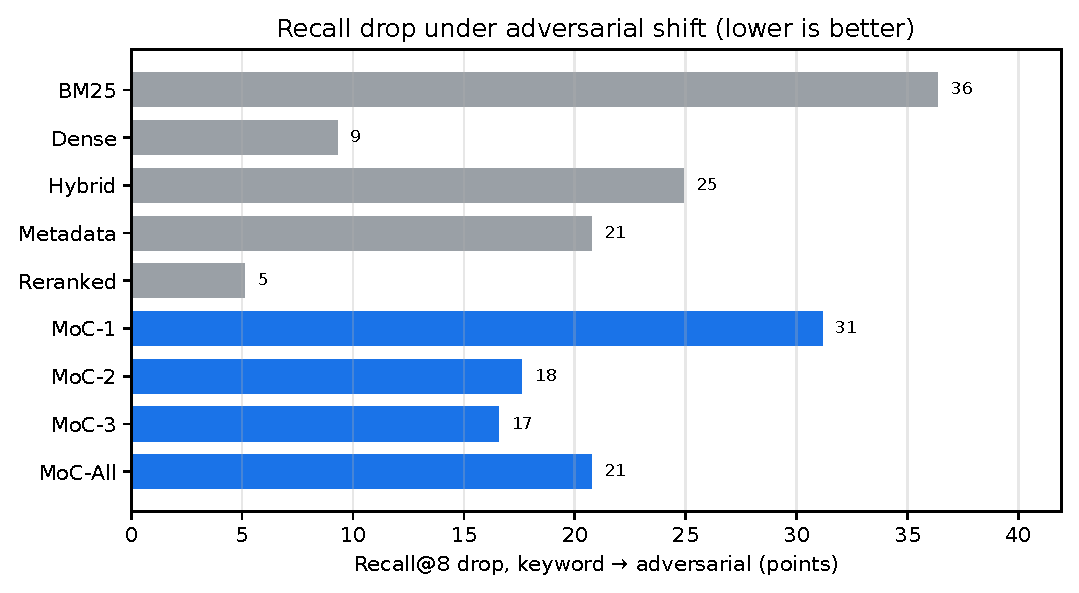
\includegraphics[width=\linewidth]{adversarial_recall_drop.pdf}
    \caption{Recall change, keyword$\to$adversarial (closer to 0 is more robust).}
    \label{fig:drop}
  \end{minipage}\hfill
  \begin{minipage}{0.49\linewidth}
    \centering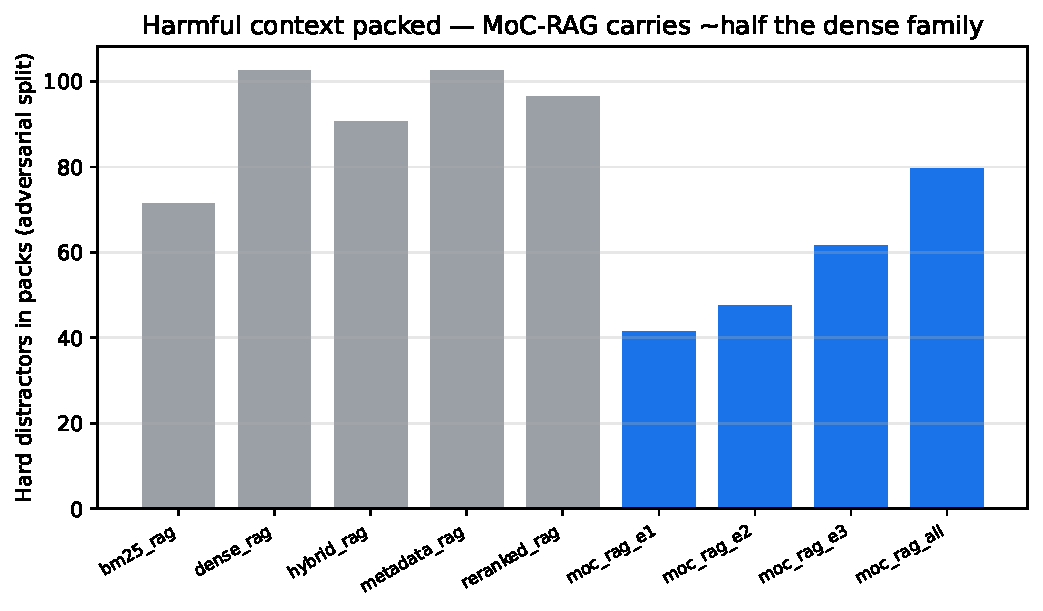
\includegraphics[width=\linewidth]{hard_distractors.pdf}
    \caption{Hard distractors packed on the adversarial split (lower is better).}
    \label{fig:hd}
  \end{minipage}
\end{figure}

\begin{figure}[t]
  \centering
  \begin{minipage}{0.49\linewidth}
    \centering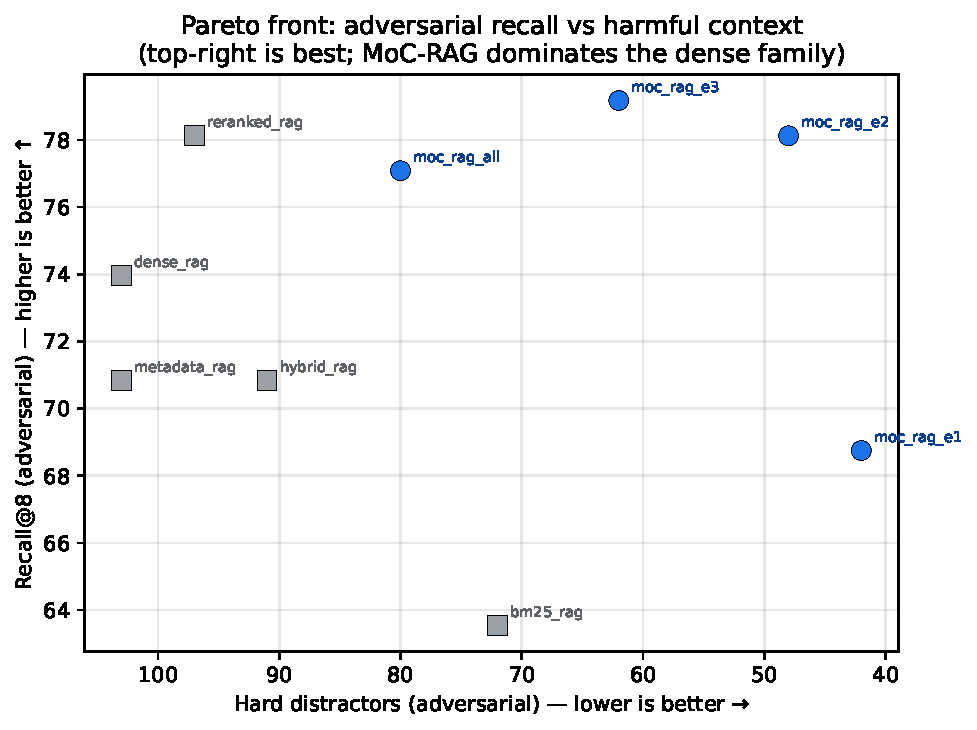
\includegraphics[width=\linewidth]{recall_vs_distractors.pdf}
    \caption{Pareto front: adversarial recall vs.\ hard distractors.}
    \label{fig:pareto}
  \end{minipage}\hfill
  \begin{minipage}{0.49\linewidth}
    \centering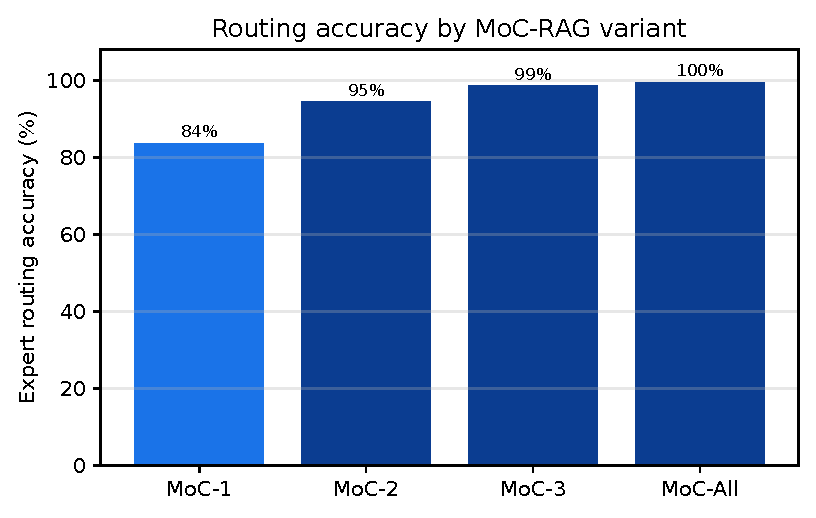
\includegraphics[width=\linewidth]{routing_accuracy.pdf}
    \caption{Expert routing accuracy by MoC-RAG variant.}
    \label{fig:route}
  \end{minipage}
\end{figure}

\paragraph{Ablation over expert fan-out.} Table~\ref{tab:abl} varies
$\mathrm{top\_experts}$. Routing accuracy rises monotonically with $k$
(Figure~\ref{fig:route}), reaching 100\% at $k{=}3$ and \texttt{all}; $k{=}2$ and
$k{=}3$ give the best recall/robustness trade-off, while $k{=}1$ minimizes hard
distractors at some recall cost. Widening to all experts recovers a flat-RAG-like
candidate pool and erodes the distractor advantage---evidence that the
\emph{selection}, not merely the typed store, drives the gains.

\begin{table}[t]
  \centering
  \caption{Ablation: MoC-RAG expert fan-out $k$ across query types.}
  \label{tab:abl}
  \begin{tabular}{l rrr r r}
\toprule
Variant & R@8 key. & R@8 par. & R@8 adv. & HD adv. & RouteAcc \\
\midrule
$k{=}1$ & 100\% & 84\% & 69\% & 42 & 75\% \\
$k{=}2$ & 96\% & 86\% & 78\% & 48 & 96\% \\
$k{=}3$ & 96\% & 89\% & 79\% & 62 & 100\% \\
all & 98\% & 85\% & 77\% & 80 & 100\% \\
\bottomrule
\end{tabular}

\end{table}

\section{Discussion}

The results support a careful, falsifiable claim rather than a sweeping one.
\textbf{BM25 is not weak}---it is the best method on keyword-aligned queries, and
a benchmark that hid this would not be credible. What changes under paraphrase
and adversarial phrasing is that surface overlap stops being a reliable signal,
and a retriever that ranks purely on words is led toward the very negatives the
benchmark plants. MoC-RAG's advantage is therefore best described as
\emph{robustness and context efficiency under typed, distractor-heavy
conditions}: it preserves more recall when lexical matching degrades, and it
keeps roughly half as much harmful context in the pack at equal token budget.

Two pieces of evidence indicate \emph{why}. First, routing accuracy tracks the
robustness gain: variants that route correctly (95--100\%) are exactly those that
resist adversarial shift, and widening to all experts---which dilutes the
routing decision---erodes the advantage. Second, the same qualitative flip
appears with the offline hashing embedder, where the dense channel is weak: the
hybrid router still routes well because its keyword, type, and scope priors do
not depend on embedding quality. The gain is thus attributable to typed
selection, not embedding strength alone.

Practically, this matches where agent memory actually lives. Real users
paraphrase, omit specifics, and ask questions whose obvious keywords point at the
wrong, outdated, or contradictory memory. In that regime, selecting the right
typed experts before retrieving is a more reliable lever than ranking a single
flat index, and the inspectability of the decision is a product feature in its
own right.

\section{Limitations and Reproducibility}

\paragraph{Limitations.} The benchmark is \emph{synthetic} and English-only.
Items and queries are template-generated, and the adversarial phrasings, while
designed to be genuinely misleading, are derived from the same templates as the
gold facts; a determined lexical baseline tuned to the templates could narrow
the gap. The dataset is also modest in scale (1{,}000 items, 600 queries). We do
not claim that MoC-RAG universally beats RAG: on keyword-aligned retrieval BM25
is at least as good, and on tasks without typed structure the routing layer adds
cost without benefit. Finally, the answer-quality column (grounded generation
with a small local model) is wired but not run end to end here; the results
above are retrieval- and context-level.

\paragraph{Threats to validity.} Because splitting is by topic and the three
variant splits are parallel, the robustness comparison is insulated from topic
leakage; but it remains a comparison within one synthetic distribution. The
hybrid router's prior weights are fixed, not learned, and were not tuned on the
test split.

\paragraph{Reproducibility.} Generation is seeded and deterministic; baselines,
metrics, figures, and tables are produced by committed scripts from committed
result artifacts (\S\ref{sec:experiments}). The dataset, the result JSONs, and a
leaderboard space are public, and the software is Apache-2.0. The next step on
the roadmap is to grow the dataset toward human-reviewed, naturally paraphrased,
real long-horizon memory, and to promote the hybrid router into the core engine
only once the gains replicate off the synthetic distribution.

\section{Conclusion}

We presented Mixture-of-Contexts RAG, a routed, inspectable retrieval
architecture for agent memory that selects typed context experts before
retrieving, and a public benchmark designed to test it where it matters: under
paraphrased and adversarial queries with planted hard negatives. The evidence is
specific and bounded. A strong lexical baseline collapses by 36 points from
keyword to adversarial queries, while MoC-RAG holds within $\sim$17 points,
overtakes that baseline on the adversarial split, and packs roughly half the
harmful context of the dense baseline family at 95--100\% routing accuracy. The
advantage is robustness and context efficiency under typed, distractor-heavy
conditions---not universal supremacy over all RAG.

This reframes the contribution from ``fewer distractors'' to a testable
robustness claim, backed by a reproducible dataset, harness, and figure
pipeline. The artifacts---software at
\href{https://github.com/agent-matrix/matrix-context}{github.com/agent-matrix/matrix-context},
dataset at
\href{https://huggingface.co/datasets/ruslanmv/moc-rag-benchmark}{huggingface.co/datasets/ruslanmv/moc-rag-benchmark},
and a leaderboard space---let anyone reproduce, contest, or extend the result.
We hope the benchmark, more than the method, is the lasting contribution: a place
where the value of typed context routing can be measured honestly.

\section*{Availability}
Software: Apache-2.0, \texttt{github.com/agent-matrix/matrix-context}. Dataset:
\texttt{ruslanmv/moc-rag-benchmark} (Hugging Face). A Zenodo DOI is minted on
tagged release (see \texttt{.zenodo.json}, \texttt{RELEASE.md}).


\bibliographystyle{plain}
\bibliography{references}

\end{document}
